\section{Architecture}

The application is structured into three modules.
Two additional modules serve to test the agent and document the application.
These modules are briefly summarized in Table \ref{tab:modules}, and their interactions are illustrated in figure \ref{fig:architecture}.

\begin{table}[h]
\centering
\begin{tabular}{|l|p{10cm}|}
\hline
\textbf{Module} & \textbf{Primary purpose} \\
\hline
\textbf{Frontend} & Desktop application for editing documents, previewing output, and chatting with the AI agent. \\
\hline
\textbf{Sidecar} & Manages local file operations, document compilation, and project configuration. \\
\hline
\textbf{Agent} & Processes user requests and makes intelligent edits to documents through sidecar tooling. \\
\hline
\textbf{User guide} & Documentation for users to install, learn, and use the application. \\
\hline
\textbf{Benchmark} & Tool for evaluating and measuring agent performance on test datasets. \\
\hline
\end{tabular}
\caption{Five modules of the Spartan Write application}
\label{tab:modules}
\end{table}

\subsection{Frontend}

Spartan Write's frontend is built with React.js \cite{react} on Tauri, enabling cross-platform development of native desktop applications for macOS, Windows, and Linux from a single TypeScript/React codebase \cite{tauri}.

\subsubsection{Development tooling and libraries}

The frontend leverages modern development tooling to ensure productivity and maintainability while maximizing accessiblity.

\begin{itemize}
    \item Tauri provides seamless integration with native system APIs while minimizing binary size, making it ideal for resource-conscious deployment across diverse user environments \cite{tauri}.
    \item Vite powers fast build times and hot module reloading during development, as well as a lightweight packaging pipeline \cite{vite}.
    \item TypeScript provides type safety across the codebase \cite{typescript}.
    \item Styling is handled by Tailwind CSS for responsive, utility-first design \cite{tailwind}.
    \item User interface components are derived from shadcn, a plug-and-play component library designed with accessibility, extensibility, and consistent visual design in mind \cite{shadcn}.
    \item The source code editor implements the Monaco Editor, which provides syntax-aware code editing with support for \LaTeX\ and other file formats \cite{monaco}.
\end{itemize}

\subsubsection{Agentic AI chat integration}

A key feature of the frontend is its integration with CopilotKit, which enables agentic chat directly within the editor \cite{copilotkit}.
The agentic chat system supports tool use for file operations, \LaTeX\ compilation, and image handling.
This tight integration allows users to request document modifications conversationally without leaving the editor.

\subsubsection{Dual-mode editor layout}

The editor employs a resizable split-panel layout that supports two complementary viewing modes.
In \emph{source view}, users see a syntax-highlighted code editor alongside a file browser for project navigation.
In \emph{preview view}, which is the default view, users see a live PDF rendering of their compiled document.
This dual-mode design provides immediate visual feedback and allows users to verify that AI-generated changes produce the desired output.

\subsubsection{Accessible interface}

Accessibility is a core design principle.
The interface includes configurable text sizing to accommodate users with vision impairments, screen reader support with live region announcements for screen reader users, a magnifier mode for enhanced visibility, and customizable PDF zoom levels ranging from 50\% to 300\%.

\subsubsection{Authentication}

The frontend integrates WorkOS AuthKit to provide secure, standards-based authentication \cite{workos}.
Users sign in via an external browser or through OAuth deeplinks, and the system manages JWT-based token refresh to maintain active sessions.
The authentication flow is designed to be seamless while adhering to security best practices.
Once authenticated, the frontend manages user credentials and provides visualization of usage data and costs.

\subsubsection{Project management}

The frontend provides a comprehensive project management interface.
Users access a dashboard to view and open recent projects.
There is an onboarding flow for new users, and a settings page displaying user profile information and usage analytics.


% TODO: Analytics and usage tracking missing in diagram
\begin{figure}[htbp]
    \centering
    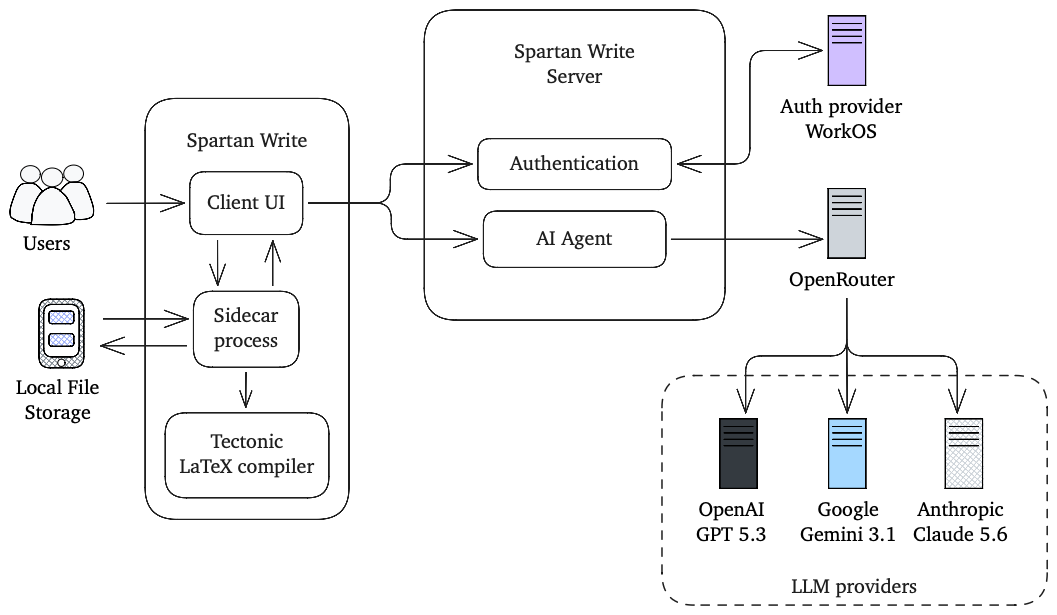
\includegraphics[width=1\linewidth]{figures/architecture.excalidraw.png}
    \caption{Architecture of the Spartan Write system}
    \label{fig:architecture}
\end{figure}

\subsection{Sidecar}

The sidecar is a local FastAPI server \cite{fastapi} bundled with the desktop application that serves as the bridge between the frontend UI and the project filesystem.
Unlike most "servers", this program runs on the users' devices alongside the client application \cite{tauri_sidecar}.
Its primary responsibility is to handle all local filesystem operations, thus keeping the cloud server stateless and focused purely on AI agent logic.

\subsubsection{Template discovery}

The sidecar provides an endpoint that lists available project templates, enabling the frontend to present users with choices when creating new projects.
This allows for easy extensibility: new templates can be added to the sidecar without requiring frontend changes.

\subsubsection{Project and file management}

The sidecar manages the complete project lifecycle on the user's machine.
When the user selects a template from the list, the program scaffolds the directory structure with the source code associated with the template.
Once a project is open, the sidecar exposes endpoints for all file operations: reading, writing, deleting, and renaming files within the project directory.
This abstraction layer ensures the frontend can safely interact with the filesystem through a controlled, authenticated API rather than direct file access.

\subsubsection{Compilation and PDF rendering}

A critical function of the sidecar is local \LaTeX\ compilation.
For this purpose, it uses Tectonic \cite{tectonic}, a lightweight \LaTeX\ compiler to compile the project.
The sidecar abstracts this program behind a convenient API that returns the compilation status and error messages to the frontend.
The compiled PDF is served back to the frontend for live preview.
The Tectonic binary is bundled alongside the sidecar itself as part of the frontend application \cite{tauri_sidecar}.
This local compilation strategy facilitates fast feedback loops and offline compilation capability without reliance on cloud-based typesetting services.


\subsubsection{Agent tool system}

The sidecar is equipped with tools for comprehensive document manipulation by the agent: reading, writing, deleting, and renaming files; listing project contents; compiling \LaTeX\ and forwarding errors if any; and managing attached images.
All file operations include path validation to prevent traversal attacks and ensure modifications remain within the project directory.
This toolset allows the agent to make changes to the project files and update the document to satisfy the user's request.

\subsubsection{Image processing}

There are two ways that the agent may choose to handle images.
Based on the user's request, the agent may decide that the image must be placed in the document, or that the image must be processed to answer a question or make a decision.
In the first case, the agent need not process the image at all, and would simply need a tool to copy it into the project directory.
Then, it could generate code to render the image within the document.
In the second case, the image would not need to be copied or stored, but instead be processed by the agent.
The sidecar provides tools for both of these purposes.

\subsubsection{Settings, health, and lifecycle}

The sidecar manages project-specific and user-level configuration, including user information, API credentials in case the user is able to provide their own API key, and authentication tokens, persisting these settings locally for quick access and offline operation.
To ensure resource efficiency, the sidecar implements parent process monitoring: if the desktop application terminates, the didecar automatically exits, preventing orphaned processes.

In summary, the sidecar encapsulates all local, filesystem-bound operations, compilation, and configuration management.
By handling these responsibilities locally, the sidecar enables offline-first workflows, fast feedback, and keeps the cloud server lightweight and stateless, focused solely on running the AI agent and managing user authentication and analytics.


\subsection{Agent}

The Agent is the cloud-based AI backbone of Spartan Write, responsible for understanding user requests and orchestrating intelligent document edits.
Built on Python FastAPI \cite{fastapi} and powered by LangGraph \cite{langgraph}, the agent manages multi-turn conversations, executes a suite of document manipulation tools, and maintains strict security boundaries.
It integrates with OpenRouter for flexible language model selection \cite{openrouter}, validates all user actions through WorkOS authentication \cite{workos}, and streams real-time feedback to the frontend while tracking usage for billing and analytics.

\subsubsection{Cloud deployment}

The agent is deployed to a trusted execution environment (TEE) on the cloud.
Its stateless architecture ensures that no persistent state is maintained between requests, enabling independent scaling and simplified deployment across multiple instances.

\subsubsection{Agent behavior \& provision}

The agent's behavior is defined using LangGraph, a framework for building stateful, multi-step AI workflows that maintain conversation context and execute complex editing logic deterministically \cite{langgraph}.
Rather than being locked to a single provider, the agent integrates with OpenRouter, a configurable LLM aggregation layer that allows selection from multiple language models and providers based on cost, performance, or capability requirements \cite{openrouter}.

\subsubsection{Authentication}

Before processing any request, the agent validates user authorization by verifying the bearer token against WorkOS \cite{workos}.
Only authenticated users are permitted to invoke the agent.

\subsubsection{Analytics \& privacy}

Every agent interaction is tracked and reported to PostHog for usage analytics, billing, and performance insights \cite{posthog}. The agent supports a "bring your own key" (BYOK) model where users provide API credentials per-request without persistent storage.
Conversation history is maintained within single sessions for multi-turn coherence but does not persist across separate chats, ensuring session isolation and data privacy.


\subsection{Benchmark}

The benchmark module is the evaluation framework for systematically assessing the agent's performance across diverse document editing scenarios.
By executing curated test datasets against the agent API and applying multi-faceted scoring metrics, the benchmark provides data-driven insights into agent capabilities, identifies performance bottlenecks, and enables comparative analysis across different models and configurations.
The goal is to select the most feasible language model and to evaluate the changes in performance across model updates.

\subsubsection{Testing workflow}

The benchmark module directly interacts with the agent server via its REST API, executing a command-line evaluation pipeline.
It systematically sends test prompts, captures agent responses and tool invocations, and generates timestamped results organized by model for comparative analysis.

\subsubsection{Curated dataset}

The benchmark uses a curated dataset of document states paired with test user prompts. 
Each dataset item represents a specific editing task, allowing systematic evaluation of the agent's capabilities across diverse, realistic scenarios.
Dataset metadata tracks task categories, complexity levels, and expected outcomes, enabling targeted analysis and identification of weaknesses in specific problem domains.

\subsubsection{Performance analysis}

Each benchmark run is scored on both objective and subjective metrics.
Objective metrics include token consumption (efficiency), tool usage count (reasoning depth), and chat duration (responsiveness).
Subjective evaluation assesses output quality, correctness of edits, and \LaTeX\ convention adherence.
The modular scoring framework allows new metrics to be added independently without modifying core evaluation logic, supporting evolving evaluation needs as the system matures.

\subsubsection{Visualization of results}

The benchmark includes a dashboard that visualizes evaluation results, aggregates scores across test cases, and enables drill-down analysis of individual runs.
This interactive interface supports identification of performance trends, failure modes, and comparative analysis across different models and configurations, making insights accessible to both researchers and product stakeholders.

\subsubsection{Reproducibility}

By maintaining consistent datasets and deterministic scoring logic, the benchmark enables reproducible evaluations across different model versions, providers, and configurations.
This reproducibility is essential for data-driven decision-making, allowing teams to confidently compare the performance of different models and settings before deploying to production.
The standardized evaluation approach also supports tracking improvements over time as the agent system evolves.

\subsection{User guide}


The user guide is built using MkDocs, a lightweight documentation framework that generates a clean, searchable website from Markdown files.
It provides a single source of truth for user-facing documentation across all supported platforms, with built-in search functionality, responsive design, and clear navigation that ensure users can quickly find answers.
The user guide covers the complete user journey, from platform-specific installation instructions for macOS, Windows, and Linux, through quick-start tutorials for first-time users, to comprehensive reference material on project management, API configuration, tips on efficient agent usage, best practices, and troubleshooting.
This breadth of content ensures users can find answers at every stage of their experience with Spartan Write.
